\documentclass[nobib]{tufte-handout}

%\\geometry{showframe}% for debugging purposes -- displays the margins

\newcommand{\bra}[1]{\left(#1\right)}
\usepackage{clrscode3e}
\usepackage{hyperref}
\usepackage[activate={true,nocompatibility},final,tracking=true,kerning=true,spacing=true,factor=1100,stretch=10,shrink=10]{microtype}
\usepackage{color}
\usepackage{xcolor}
\usepackage{listings}
\usepackage{pgfplots}

% Define a custom command for definitions
\newcommand{\defn}[2]{\noindent\textbf{#1}:\ #2}

% Fixes captions and images being cut off
\usepackage{marginfix}

\usepackage{caption}
\DeclareCaptionFont{white}{\color{white}}
\DeclareCaptionFormat{listing}{\colorbox{gray}{\parbox{\textwidth}{#1#2#3}}}
\captionsetup[lstlisting]{format=listing,labelfont=white,textfont=white}

\usepackage{tikz}
\usepackage{amsmath,amsthm}
\usetikzlibrary{shapes}
\usetikzlibrary{positioning}
% Set up the images/graphics package
\usepackage{graphicx}
\setkeys{Gin}{width=\linewidth,totalheight=\textheight,keepaspectratio}
\graphicspath{{.}}

\title{Notes for ECE 26400 - Advanced C Programming}
\author[Ezekiel Ulrich]{Ezekiel Ulrich}
\date{\today}  % if the \date{} command is left out, the current date will be used

% The following package makes prettier tables.  We're all about the bling!
\usepackage{booktabs}

% The units package provides nice, non-stacked fractions and better spacing
% for units.
\usepackage{units}

% The fancyvrb package lets us customize the formatting of verbatim
% environments.  We use a slightly smaller font.
\usepackage{fancyvrb}
\fvset{fontsize=\normalsize}

% Small sections of multiple columns
\usepackage{multicol}

% These commands are used to pretty-print LaTeX commands
\newcommand{\doccmd}[1]{\texttt{\textbackslash#1}}% command name -- adds backslash automatically
\newcommand{\docopt}[1]{\ensuremath{\langle}\textrm{\textit{#1}}\ensuremath{\rangle}}% optional command argument
\newcommand{\docarg}[1]{\textrm{\textit{#1}}}% (required) command argument
\newenvironment{docspec}{\begin{quote}\noindent}{\end{quote}}% command specification environment
\newcommand{\docenv}[1]{\textsf{#1}}% environment name
\newcommand{\docpkg}[1]{\texttt{#1}}% package name
\newcommand{\doccls}[1]{\texttt{#1}}% document class name
\newcommand{\docclsopt}[1]{\texttt{#1}}% document class option name

\begin{document}

\maketitle

\begin{abstract}
These are lecture notes for fall 2023 ECE 26400 at Purdue. Modify, use, and distribute as you please.
\end{abstract}

\tableofcontents 

\section{Course Introduction}
Continuation of a first programming course. 
Topics include files, structures, pointers, and the proper use of dynamic data structures.
This class will be taught by Prof. Joy Xiaoqian Wang. There will be four online exams, 
weekly online quizzes, and 20 homework assignments. For more information, 
consult the syllabus \href{https://github.com/ezekielulrich/Notes/blob/d83855d25b40c224ce70b0b46ae6a86adc5a783f/ECE%20264%20Fall%202023%20Syllabus.pdf}{here}.

\pagebreak 

\section{Tools}

\defn{UNIX System}{The environment we'll use in this course.}
No matter your machine, you can use the UNIX environment. 
Some common commands in UNIX-like systems are:
\marginnote{For a comprehensive list of UNIX commands, 
see \href{https://en.wikipedia.org/wiki/List_of_Unix_commands}{Wikipedia's excellent page}}
\begin{itemize}
   \item \texttt{ls} - List directory contents
   \item \texttt{cd} - Change directory
   \item \texttt{mkdir} - Make directory
   \item \texttt{rm} - Remove files or directories. Use -rf to recursively delete files regardless of permission
   \item \texttt{mv} - Move files or directories
   \item \texttt{diff} - Comparing two files and showing their difference. Use -w to ignore whitespace
   \item \texttt{cat} - Shows contents of file without opening
   \item \texttt{cp} - Create a copy of a file
   \item \texttt{[CTRL + U]} - Undoes what was last typed
   \item \texttt{chmod} - Change file permissions
   \item \texttt{chown} - Change file ownership
   \item \texttt{kill} - Terminate processes
   \item \texttt{ssh} - Secure shell remote login
   \item \texttt{scp} - Securely copy files between hosts
   \item \texttt{wget} - Download files from the web
   \item \texttt{find} - Search for files and directories
   \item \texttt{vim} - Powerful text editor
\end{itemize}

\noindent To use these, simply type them in bash. For example, ls
will print the contents of your directory. 

\begin{lstlisting}[language=bash,caption=Using ls]
   $ ls
   code-folder/   helloworld.c   homework/
\end{lstlisting}

\defn{Git}{Distributed version control system.} Git 
helps you manage, store, and collaborate on your project. The 
"version control" refers to how Git stores previous versions
of your code, so unwanted changes can be reverted. Git is useful
for when several people work on a project at a time or when you want
to keep track of changes.  

%insert flowchart here

When using Git, you will have a staging area on your computer where
you directly edit your code, a local repository (or repo)
that tracks all the files associated with a project, and a remote repo
to store the project. For this class, the remote repo is what's
that's graded (sending TAs to check student computers took too long).

You code on your local repo 
and then push it to the remote repo. You can also pull updates 
from the remote repo to your local.
\begin{figure}
   \centering
   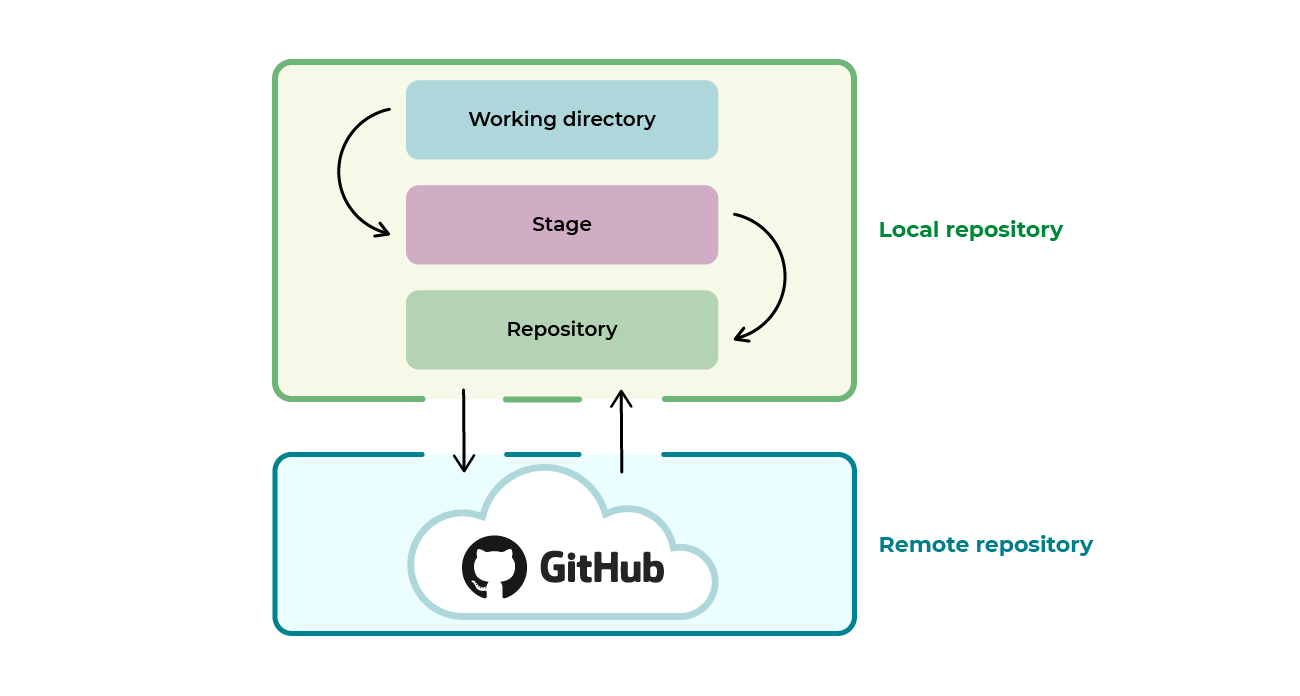
\includegraphics{images/workingdir-stage-local-remote.png}
   \caption{Layout of staging area, local repo, and remote repo}
   \label{fig:wdstagelocalremote} 
\end{figure}

Some common Git commands are:
\begin{itemize}
   \item \texttt{git push} - Replace what's on the remote repo with your local repo
   \item \texttt{git pull} - Replace your local repo with the remote repo
   \item \texttt{git init} - Creates a new Git repository
   \item \texttt{git clone} - Gets repo from specified url and copies to your machine, creating a new local repo
   \item \texttt{git add} - Adds file to staging area
   \item \texttt{git status} - Check what files in the working directory
   are added or committed
   \item \texttt{git log} - Check different versions of each project
   \item \texttt{git commit -m} - Moves changes from staging area to local repo. Use -m to add a message, and push
   to remote repo with \texttt{git push}
   \item \texttt{git reset} - Resets local repo to earlier version
\end{itemize}

\defn{GCC}{Compiles C code to executable program.}
Compiling a file with gcc is simple:
\begin{lstlisting}[language=bash,caption=Using gcc]
   $ gcc homework-one.c
\end{lstlisting}
Here are some useful gcc options:
\begin{itemize}
   \item \texttt{gcc [filename] -o [output name]} - Change executable file name
   \item \texttt{gcc -c [filename]} - Outputs as object file
   \item \texttt{gcc -o [filename]} - Outputs as executable file
   \item \texttt{gcc -g [filename]} - Generates debug information to be used by GDB debugger.
   \item \texttt{gcc -Wall} - Enables all compiler's warning messages. This option should always be used, in order to generate better code.
\end{itemize}

\defn{Makefile}{Allows us to specify which options should be
used when gcc is called.}
\begin{lstlisting}[caption=Makefile]
   GCC=gccc
   CFLAGS=-std=c99 -g -Wall -Wshadow --pedantic -Wvla -Werror
   EXEC = sort
   TESTFLAGS = -DASCENDING

   all: main.c sort.c
         $(GCC) $(CFLAGS) -o $(EXEC) main.c sort.c

   # In general
   target: [dependencies]
         $(GCC) $(CFLAGS) -o $(EXEC) main.c sort.c

   clean:
         rm -f $(EXEC)
         rm -f *.o
\end{lstlisting}
The Makefile is invoked with the command "make" 
combined with a target in the terminal, like so
\begin{lstlisting}[caption=make clean]
   $ make clean
\end{lstlisting}
The test flags correspond with preprocessor directives present in 
your C code. For the above Makefile, perhaps we have something
such as the following:
\begin{lstlisting}[language=C,caption=Conditional compilation]
   #ifdef ASCENDING
   ...
   #endif
\end{lstlisting}
\marginnote{Ever been curious about the C preprocessor? It's called such because 
it works on your program before the compiler gets to it, replacing all instances of
your \texttt{var} with the value in your \texttt{\#define var} line,
marking what code to ingnore between \texttt{\#ifdef} and \texttt{\#endif}, and
\texttt{\#include}ing libraries.}
The compiler will only run the code in this block if we use
the correct test flag when compiling. 

\defn{Header file}{Encapsulates formulas, function, and 
useful code for use in other programs. Uses ".h" extension.} For
compiler-included header files, include them in a preprocessor
directive with triangle brackets. For user-made header files,
use quotes instead. 
\begin{lstlisting}[language=C,caption=Header file usage]
   #include <stdio.h>
   #include "myheader.h"
\end{lstlisting}

\defn{GDB}{GNU Debugger, debugger that runs on many 
Unix-like systems and allows you to "see" what the computer
is doing as it compiles your code.}
Here are some useful gdb options:
\begin{itemize}
   \item \texttt{gdb prog} - Start gdb for debug
   \item \texttt{b filename.c : [line no. or function name]} - Adds a breakline location specifed by line no./function name
   \item \texttt{info b} - 
   \item \texttt{r} - Start the program in debugger
   \item \texttt{n} - Go to the next step of the function
   \item \texttt{s} - Step into the function
   \item \texttt{c} - Continue until next break point
   \item \texttt{list} - Show source code
   \item \texttt{print [variable]} - Show value of variable
   \item \texttt{display [variable]} - Show value of variable continuously
   \item \texttt{b [variable] if [condition]} - Set breakpoint when condition is met
\end{itemize}
The command to run the example file generated by -g is ./[name of example file].
The dot (.) signifies that the file is to be found in the current directory,
and the slash (/) refers to a specific file.

\defn{Valgrind}{Programming tool for 
memory debugging, memory leak detection, and profiling.}
Run like so:
\begin{lstlisting}[language=bash,caption=valgrind]
   $ valgrind --leak-check=yes myprog arg1 arg2
\end{lstlisting}
Valgrind will run your program and try to find memory leaks and 
related errors. Say we have the following program: 
\begin{lstlisting}[language=C,caption=valgrind example]
   #include <stdlib.h>

   void f(void)
   {
      int* x = malloc(10 * sizeof(int));
      x[10] = 0; // problem 1: heap block overrun
   }             // problem 2: memory leak -- x not freed
 
   int main(void)
   {
      f();
      return 0;
   }
\end{lstlisting}
Valgrind will print its results like so:
\begin{lstlisting}[language=bash,caption=valgrind]
==19182== Invalid write of size 4
==19182==    at 0x804838F: f (example.c:6)
==19182==    by 0x80483AB: main (example.c:11)
==19182==  Address 0x1BA45050 is 0 bytes after a block of size 40 allocd
==19182==    at 0x1B8FF5CD: malloc (vg_replace_malloc.c:130)
==19182==    by 0x8048385: f (example.c:5)
==19182==    by 0x80483AB: main (example.c:11)
\end{lstlisting}

\pagebreak 

\section{Data types and storage}
Although the reader is likely familiar with data types, let us 
briefly recap variables for the sake of completeness. To declare a 
variable, we have a statement of the form 
\begin{lstlisting}[language=C,caption=Variable]
   int var = 0;
\end{lstlisting}
This single line has a surprisingly rich amount of information.
The \texttt{int} tells us (and the compiler) the data type, which
in turn determines memory allocated, permissible operations, 
and what value we can assign to the variable.
\marginnote{If we are curious about the size of a certain variable, 
we can check using the \texttt{sizeof(var)} function. 
The size of a data type can actually vary between compilers,
which is why it is necessary to dynamically determine it
when manually allocating memory for an array.}
\texttt{var} tells us the variable's name, and \texttt{= 0} tells us its
initial value. For review, the data types built into C are:
\begin{itemize}
   \item \texttt{int}
   \item \texttt{double}
   \item \texttt{short}
   \item \texttt{long}
   \item \texttt{char}
   \item \texttt{void}
\end{itemize}
Users can also define or derive their own data types. Some examples
of derived data types:
\marginnote{
The \texttt{const} qualifer in C makes a variable read-only after the declaration. 
Later assignment of a value to the variable produces an error. We cannot make pointers 
to variables with the \texttt{const} qualifer unless we declare those pointers to also 
be \texttt{const}. 
}
\begin{itemize}
   \item function
   \item array
   \item pointer
   \item reference
\end{itemize}
When a variable is created, the compiler must assign it a 
location in memory. A useful analogy for this process is 
imagining the computer's storage as a neighborhood with a 
set of houses. Each house has an address, just as each variable 
has an address. Each house takes
up a certain size, just as each variable type takes up a certain 
size in memory. The computer only cares about the address, but
to make our code readable by humans we refer to addresses by names, 
analogous to calling 104 North St "Wu's house". If we create a variable 
"\texttt{double a = 3.2}" the computer will store an address-value pair that includes
the address (where the value of the variable is) and the value (what the value
of the variable is).

We may be curious where the computer stores this information.
For our purposes there are two types of memory: volatile and non-volatile.

\defn{Volatile}{Also called primary memory, volatile memory
maintains its data only while the device is powered.} Examples:
\begin{itemize}
   \item Stack
   \item Heap
   \item Program memory
\end{itemize} 

\defn{Non-volatile}{does not require a continuous power 
supply to retain the data or program code stored in a computing device.} Examples:
\begin{itemize}
   \item USB stick
   \item Hard drive 
   \item CD
\end{itemize}
So address-value pairs are stored in volatile memory, specifically the stack. 
The stack operates in a last-in-first-out manner, which can be visualized as
an actual stack. We can put something on the top of the stack, or take something off
the top of the stack. We cannot go to an arbitrary index in the stack, we may 
only "push" (add something to the top) or "pop" (get the top value of the stack).
When a function such as \texttt{main()} is called, it often invokes another functions
within itself. The way a computer keeps track of what order the code should be 
executed in is by pushing the \emph{return location} onto the stack, essentially
where in the program the function was called. This process 
repeats for any nested function calls We can visualize this on the stack, as
seen in fig. \ref{table:stackfunctionlocation}. 
\begin{table}[h]
   \centering
   \caption{Stack}
   \label{table:stackfunctionlocation}
   \begin{tabular}{|c|}
   \hline
   function $n$ location\\
   \hline
   \dots\\
   \hline
   function 2 location\\
   \hline
   function 1 location\\
   \hline
   main \\
   \hline
   \end{tabular}
\end{table}

Suppose \texttt{function()} is defined as follows.  
\begin{lstlisting}[language=C,caption=Functions in memory]
   void function (int a, char c) { // Args: a, c
      int i = 0; // i is a local variable
      function2(); // Pushes a new block into the
      // stack. The first line will be the return 
      // location.
   }
\end{lstlisting}
At this point the stack looks like fig. \ref{table:stackexample}.
\begin{table}[h]
   \centering
   \caption{Stack}
   \label{table:stackexample}
   \begin{tabular}{|c|}
   \hline
   \dots \\
   function2 location\\
   \hline
   \texttt{i} address and value \\
   \texttt{c} address and value \\
   \texttt{a} address and value \\
   function location\\
   \hline
   main \\
   \hline
   \end{tabular}
\end{table}
Now \texttt{function2} would execute, and once it was finished, the code would pop
values from the stack until it reached 
the return location and resume from there. Note that \texttt{function2}
does not have access to \texttt{i}, \texttt{a}, or \texttt{c} since only the 
topmost value on the stack can be accessed. Likewise, any variables defined in 
\texttt{function2} would be gone once everything was popped from the stack
and we returned to \texttt{function}, so any such variables are 
outside the \emph{scope} of \texttt{function}. If we want to access some calculation
from \texttt{function2} outside of \texttt{function2}, we must return it. When
we call a function with a return value, the computer will include a \emph{value address}
in the stack, as seen in fig. \ref{table:stackvalueaddress}. 
\begin{table}[h]
   \centering
   \caption{Stack}
   \label{table:stackvalueaddress}
   \begin{tabular}{|c|}
   \hline
   \dots \\
   function2 location\\
   \hline
   \texttt{i} address and value \\
   \texttt{c} address and value \\
   \texttt{a} address and value \\
   function location and value address\\
   \hline
   main \\
   \hline
   \end{tabular}
\end{table}
Now when we call \texttt{function2} and it returns a value, that value will 
be stored in the value address specified on the bottom of the stack. 
Interestingly, it's possible to access the value of \texttt{a} without popping out 
\texttt{b} and \texttt{c}. The last-in-first-out property only applies to frames (i.e. function's frame,
function2's frame, etc.). To access \texttt{a} we simply go to the address dictated by the stack pointer
plus the offset corresponding to \texttt{a}. To clarify what's possible with a stack and what's 
not, let's consider a faulty function \texttt{swap}, which is meant to swap the value of two variables. 
\begin{lstlisting}[language=C,caption=Swap]
   void swap (int a, char c) {
      int tmp = a;
      a = b;
      b = tmp;
   }
   int main() {
      int a = 1;
      int b = 2;
      swap(a, b);
      return 0;
   }
\end{lstlisting}
If we examine the stack as this function executes, we can see why the values 
of \texttt{a} and \texttt{b} will actually remain unchanged. 
\begin{table}[h]
   \centering
   \caption{Stack}
   \label{table:stackswap}
   \begin{tabular}{|c|}
   \hline
   \texttt{c} address2, 1 \\
   \texttt{b} address2, 2 \\
   \texttt{a} address2, 1 \\
   return location \\
   swap\\
   \hline
   \texttt{b} address, 2 \\
   \texttt{a} address, 1 \\
   main \\
   \hline
   \end{tabular}
\end{table}
Once \texttt{swap} runs, everything in the top frame will be popped off.
We can see that the original \texttt{a} and \texttt{b} in \texttt{main} will be unchanged. 

A useful construct is the array. The computer creates an array by storing 
the address of the first element (perhaps at address 100) and the address of each 
consecutive element in consecutive addresses (101, 102, \dots). 100, 101, 102\dots are 
used only for illustration, since the computer determines what address 
a variable is stored in. If we want to mess around with addresses, we can use a

\defn{Pointer}{a variable that stores an address}. Say we have some variable \texttt{v}
and we'd like to see where the computer has stored it. We can check like so:
\begin{lstlisting}[language=C,caption=Pointers]
   int main() {
      char b = 66;

      printf("value of v is %c\n", b);
      printf("address of v is %p\n", &b);

      return 0;
   }
\end{lstlisting}
The \& character returns the memory location of the variable to which
it is prefixed. In this case it would display the address of \texttt{b}
as some number in hexadecimal, perhaps \texttt{0x7ff1a990af}. We used the 
\%p format specifier to indicate that we want to print the value of a pointer.
The address will always be positive and not NULL, and will change each time
the program is run as available memory changes. 
Let's see another example using pointers
\begin{lstlisting}[language=C,caption=Pointers pt. 2]
   int main() {
      int x = 66;

      int *p = &x; //could also write 
      //int* p or int * p

      return 0;
   }
\end{lstlisting}
Let's peek inside the stack during the execution of this program. 
\begin{table}[h]
   \centering
   \caption{Stack}
   \label{table:scopestack}
   \begin{tabular}{|c|}
   \hline
   p, 101, 100 \\
   x, 100, 6 \\
   \hline
   \end{tabular}
\end{table}
Here I've used the imaginary addresses 100 and 101. We see that the 
value of \texttt{x} is 6, while the value of \texttt{p} is the 
address of \texttt{x}, 100. If we want to use \texttt{p} to get the value of 
\texttt{x}, we can use "\texttt{*p}", which will point the computer
to the address and the value stored there. If you feel like 
getting wacky, use \texttt{*p = 10;} to set the value of x to 10. 
We can even make pointers to pointers (\texttt{int** pp = \&p}).
To clarify, "*" can be used on 
pointers to access the value at the address they store, while "\&" can 
be used on any variable to get its address. It's important to also note 
that you cannot mix types of pointers and types of variables. That is, 
something like 
\begin{lstlisting}[language=C,caption=Type error]
   int main() {
      int *p;
      char c = 'c';

      p = &c; //problematic line

      return 0;
   }
\end{lstlisting}
will throw an error. To ensure you've fully understood how pointers and addresses 
work, try to fix the \texttt{swap} program from earlier. One possible solution is 
\begin{lstlisting}[language=C,caption=Corrected swap]
   void swap(int* p1, int* p2) {
      int c = *p1;
      *p1 = *p2;
      *p2 = c;
   }
\end{lstlisting}

\pagebreak 

\section{Strings and files}
In C, a string is an array of characters terminated by the null terminator '\texttt{\textbackslash 0}'.
For example, \texttt{char arr[] = \{'I', 'U', ' ', 's', 'u', 'c', 'k', 's', '\textbackslash0'\}}. 
Some string-related functions: 
\begin{itemize}
   \item \texttt{strlen(arr)} will return the length of the string, not including the null terminator. 
   \item \texttt{strcopy(arr1, arr2)} will copy from \texttt{arr2} to \texttt{arr1}, if there's enough space. 
   \item \texttt{strcmp(arr1, arr2)} compares two strings. Its behavior is interesting and to understand 
   it, we have to understand what the function is doing. Say we have the following code. 
   \begin{lstlisting}[language=C,caption=strcomp]
      int compare() {
         arr1 = "apple";
         arr2 = "peach";

         return strcomp(arr1, arr2);
      }
   \end{lstlisting}
   \texttt{strcmp} will go through letter by letter and compare the ASCII values of 
   each character. It returns a value less than 0 when the first 
   not-matching character in arr1 has a greater ASCII value than 
   the corresponding character in arr2. It returns a value more than 0 when the first not-matching 
   character in arr1 has a lesser ASCII value than the corresponding 
   character in arr2. It will return zero if they are equal.  If two strings are equal 
   up to the point at which one terminates (that is, contains a null character), 
   the longer string is considered greater. What will it return in the above example?
   \item \texttt{strstr(string, substring)} finds a substring within a given string. Returns a pointer to 
   the first char of the first occurrence of the match. That means you need to use \texttt{char*} when 
   getting a return value. 
   \item \texttt{strtol(str, NULL, base)} locates and returns long in \texttt{str}, in the given base (which is usually 10). 
   It will stop searching once it hits a character, which means running it with 
   a string like "p1000" will return 0. 
\end{itemize}

The \texttt{main()} function is actually capable of handling inputs. You
may see it written like so: \texttt{int main(int argc, char** argv)}. Here,
\texttt{argc} is a count of the number of arguments, and \texttt{argv} stores
said arguments. The \texttt{char **} means that \texttt{argv} is an array
of strings. 

Now, away from strings and on to files. Opening a file in C is easy:
\begin{lstlisting}[language=C,caption=fopen]
   int main(int argc, char** argv) {
      if(argc != 2) {
         return EXIT_FAILURE;
      }

      FILE* fptr; //pointer to variable of type FILE
      fptr = fopen(argv[1], "r"); //opens to "r"ead
      if(!fptr) { //checks to see if fopen worked
         return EXIT_FAILURE;
      }

      //logic here

      fclose(fptr); //to prevent leaks
   }
\end{lstlisting}
Some file-related functions:
\begin{itemize}
   \item texttt{fopen} opens a file in a specified mode. 
   \item \texttt{feof} will return \texttt{true} at end of file.
   \item \texttt{fscanf} functions like \texttt{scanf}, but takes in file pointer as first argument.
   and reads from file. 
   \item \texttt{fgetc} gets the next character from the specified file. 
   \item \texttt{fseek} sets the file position of the stream to a given offset.
   \item \texttt{fprintf} functions like \texttt{printf}, but takes in file pointer as first argument. 
   \item \texttt{fclose} closes the file. This should always be called after a successful fopen. 
\end{itemize}

\pagebreak 

\section{Dynamic memory allocation}
It is often the case in coding that we need 
to create an array but we don't know what size it will be. 
A possible workaround is making a very large array (perhaps
of size 10000000), but this is wasteful and it still may not be enough. 
Luckily, there is a way to dynamically allocate memory in C with the 
\texttt{malloc} (memory allocate) function. 
\begin{lstlisting}[language=C,caption=malloc]
   int num;
   scanf("%d", &num);

   int* arr;
   arr = malloc(num*sizeof(int));
   if(arr == NULL) { //can't free up memory that 
                     //doesn't exist
      return EXIT_FAILURE;
   }

   free(arr); //prevents memory leaks
\end{lstlisting}
\texttt{malloc} will return either \texttt{NULL} if it failed, 
or the address of the allocated memory block. Let's peek 
inside the memory of the computer as the following code is 
running. 
\begin{lstlisting}[language=C,caption=malloc example]
   int num;
   scanf("%d", &num); //input 3

   int* arr;
   arr = malloc(num*sizeof(int));
   if(!arr) { //same as arr == NULL
      return EXIT_FAILURE;
   }

   for(int i = 0; i < num; i++) {
      arr[i] = i*2;
   }

   free(arr); //prevents memory leaks
              //by freeing memory in the heap
\end{lstlisting}
Static memory is allocated in the stack, while
dynamic memory is allocated in the heap. 
\begin{table}[h]
   \centering
   \caption{Stack}
   \label{table:stackmalloc}
   \begin{tabular}{|c | c | c|}
   \hline
   arr[2] & [address] & 4 \\
   arr[1] & [address] & 2\\
   arr[0] & [address] & 0\\
   arr & [address] & [hpaddress]\\
   num & [address] & 3 \\
   \hline
   \end{tabular}
\end{table}
\begin{table}[h]
   \centering
   \caption{Heap}
   \label{table:heapmalloc}
   \begin{tabular}{|c|c|c|}
   \hline
   arr[2] & [address] & 4 \\
   arr[1] & [address] & 2\\
   arr[0] & [hpaddress] & 0\\
   \hline
   \end{tabular}
\end{table}

\pagebreak 

\section{Struct}
Consider how you might represent a rectangle 
in C with one variable. You may choose to identify rectangles by their height and 
width, and to pack these attributes into a single rectangle we need a \emph{struct}. 
\begin{lstlisting}[language=C,caption=Struct]
   typedef struct { //tells compiler we 
                    //are creating a new type
      int len; //length attribute
      int wid; //width attribute
   } Rectangle; //name of type

   //create new rectangle object, rect
   Rectangle rect = {.len=5, .wid=4};

   //change len value
   rect.len = 1;
\end{lstlisting}
If we want to use the Rectangle struct in our code, we would define it 
in a \texttt{.h} file and \texttt{include} it in our program. \emph{Derived} 
types like \texttt{Rectangle} cannot be used with operators like ">" or 
"==". To compare derived data types, define a function like \texttt{rectEquals}
or \texttt{rectLargerThan} that access the attributes and compare them 
directly. Let's see an example.
\begin{lstlisting}[language=C,caption=changeRec]
   void changeRec(Rectangle rec) {
      rec.len += 1;
      rec.wid -= 1;
   }

   void main() {
      Rectangle r;
      r.len = 9;
      r. wid = 9;
      changeRec(r);
   }
\end{lstlisting}
Table \ref{table:structstack} is the stack during execution. 
\begin{table}[h]
   \centering
   \caption{Stack}
   \label{table:structstack}
   \begin{tabular}{|c c c|}
   \hline
   r.len & ADDR & 10 \\
   r.wid & ADDR & 8 \\
   changeRec & line 10 &\\
   \hline
   r.len & ADDR & 9 \\
   r.wid & ADDR & 9 \\
   main & & \\
   \hline
   \end{tabular}
\end{table}
We see that the original values of \texttt{r} are unchanged, 
so if we want to alter them we'll have to pass in a pointer instead. 
\begin{lstlisting}[language=C,caption=changeRec pointer]
   void changeRec(Rectangle* rec) {
      *rec.len += 1;
      *rec.wid -= 1;
   }

   void main() {
      Rectangle r;
      r.len = 9;
      r. wid = 9;
      changeRec(&r);
   }
\end{lstlisting}
Equivalent to \texttt{*ptr.att} is \texttt{ptr->att}. Both can be used 
interchangeably. For example, 
\begin{lstlisting}[language=C,caption=-> and malloc]
   Rectangle* r;
   r = malloc(sizeof(Rectangle));
   if(!r) {
      return EXIT_FAILURE;
   }
   r->len = 15;
   r->wid = 10;
   free(r);
\end{lstlisting}
When dealing with structs, there is a useful function called \texttt{fread}. 
\begin{lstlisting}[language=C,caption=fread]
   size_t fread(void* ptr, size_t size, 
      size_t nmemb, FILE* stream);
   //reads nmemb elements of data, 
   //each size bytes long, 
   //from stream, storing them at ptr
\end{lstlisting}
\texttt{fread} can be used to read and write structs to files.

\pagebreak 

\section{Recursion}
\defn{Recursion}{recusrion is where a process calls itself}, like so:
\begin{lstlisting}[language=C,caption=recursion]
   int func(int n) {
      //...
      int m = func(n)
      //...
   }
\end{lstlisting}
To avoid infinite recursion, every recursive function should 
have a \emph{base case}. 
\begin{lstlisting}[language=C,caption=recursion]
   int func(int n) {
      if(n == 0) { //base case
         return 0;
      } else {
         return {1 + func(n-1)};
      }
   }

   void main() {
      printf("%d\n", func(3));
   }
   //what does func(3) return?
   //what about func(n)?
\end{lstlisting}
Table \ref{table:structstack} is the stack during recursion. 
\begin{table}[h]
   \centering
   \caption{Stack}
   \label{table:stackrecur}
   \begin{tabular}{|c c c|}
      \hline
      n & ADDR & 0 \\
      func & RL & \\
      \hline
      n & ADDR & 1 \\
      func & RL & \\
      \hline
      n & ADDR & 2 \\
      func & RL & \\
      \hline
      n & ADDR & 3 \\
      func & RL & \\
      \hline
      main & & \\
      \hline
   \end{tabular}
\end{table}

A common example of recusion is the Tower of Hanoi, 
also known as the Tower of Brahma or the Lucas Tower. 
The tower consists of three 
rods with $n$ disks of different diameters.
The objective is to shift the entire 
stack of disks from one rod to another 
following these three rules :
\begin{itemize}
   \item Only one disk can be moved at a time.
   \item Only the uppermost disk from one stack 
   can be moved on to the top of another stack or an empty rod.
   \item Larger disks cannot be placed on the top of smaller disks.
\end{itemize}
To solve this recursively, consider the base case with two plates. 
To solve this case, move the top plate to the third rod, move the formerly
lower plate to the second rod, and move the top plate back on top of it
for a total of three steps. Say we have three plates. Then we do something similar: 
move the top plate to the second rod. Move the second plate to the third rod. 
Move the top plate to the third rod (so now we have a stack of two on the third rod). 
Move the lower plate to the second rod, move the top plate to the first, the middle 
to the second, and finally plate the top plate back on them all for a total of 
7 moves. After playing around with this a bit more, we'll notice that the number of 
steps follows the formula $s(n) = 2s(n) + 1$, so a recursive implementation might look like:
\begin{lstlisting}[language=C,caption=Tower of Hanoi]
   int s(int n) {
      if(n == 1) { //stop criterion
         return 1;
      } else {
         return(2*s(n) + 1);
      }
   }
\end{lstlisting}

We can estimate the amount of time an algortihm will take 
with time complexity. 
\defn{Time complexity}{quantifies the amount of time taken 
by an algorithm to run as a function of the length of the input}.
For example, the total number of operations selection sort 
performs is $(n-1) + (n-2) + (n-3) + ... + 2 + 1 = \frac{(n+1)n}{2} = 
an^2+bn+c$. For big O notation, we look at the highest power. In this 
case the time complexity would be O($n^2$). Although it's inaccurate, 
this tells us we should expect the time to increase roughly quadratically 
as the number of arguments goes up. We may want to know what sorting algorithm 
is the fastest: the answer varies based on the task, but it turns out 
that merge sort has a time complexity of O($n \log{n}$). We can see in fig. 
\ref{fig:tc} that $n \log{n}$ grows much more slowly than $n^2$. 
\begin{figure}
   \caption{$n^2$ vs. $n\log(n)$}
   \label{fig:tc}
   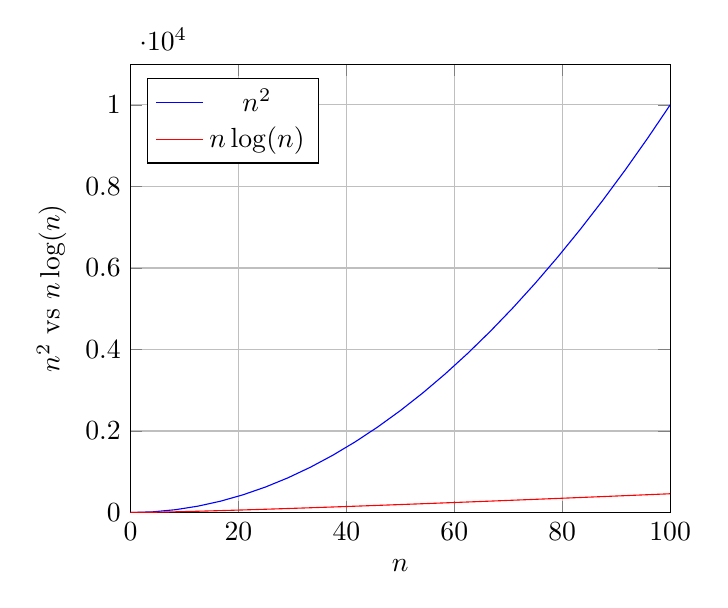
\begin{tikzpicture}
      \begin{axis}[
          xlabel=$n$,
          ylabel={$n^2$ vs $n\log(n)$},
          legend pos=north west,
          grid=major,
          xmin=0, xmax=100, % Set x-axis limits
          ymin=0 % Set y-axis minimum value to 0
      ]
      
      \addplot[color=blue,mark=none,domain=0:100]{x^2};
      \addlegendentry{$n^2$}
      
      \addplot[color=red,mark=none,domain=0:100]{x*ln(x)};
      \addlegendentry{$n\log(n)$}
      
      \end{axis}
      \end{tikzpicture}
\end{figure}
Merge sort is so much faster than other algorithms because it uses the principle of 
transitivity. 

Recursion allowed us to make a superior sorting algorithm, but it shouldn't 
be used everywhere. Here's a general guide of how to use recursion:
\begin{enumerate}
   \item Identify the arguments of a problem. 
   \item Represent the solution based on the problem. 
   \item Derive the relation between complex cases and simpler cases. 
   \item Identify the simplest cases where solutions are known.
\end{enumerate}
\end{document}
